\documentclass[10pt,]{article}
\usepackage{lmodern}
\usepackage{amssymb,amsmath}
\usepackage{ifxetex,ifluatex}
\usepackage{fixltx2e} % provides \textsubscript
\ifnum 0\ifxetex 1\fi\ifluatex 1\fi=0 % if pdftex
  \usepackage[T1]{fontenc}
  \usepackage[utf8]{inputenc}
\else % if luatex or xelatex
  \ifxetex
    \usepackage{mathspec}
  \else
    \usepackage{fontspec}
  \fi
  \defaultfontfeatures{Ligatures=TeX,Scale=MatchLowercase}
\fi
% use upquote if available, for straight quotes in verbatim environments
\IfFileExists{upquote.sty}{\usepackage{upquote}}{}
% use microtype if available
\IfFileExists{microtype.sty}{%
\usepackage{microtype}
\UseMicrotypeSet[protrusion]{basicmath} % disable protrusion for tt fonts
}{}
\usepackage[margin=1in]{geometry}
\usepackage{hyperref}
\hypersetup{unicode=true,
            pdftitle={Machine Learning - the basics in R},
            pdfauthor={Jan-Philipp Kolb},
            pdfborder={0 0 0},
            breaklinks=true}
\urlstyle{same}  % don't use monospace font for urls
\usepackage{color}
\usepackage{fancyvrb}
\newcommand{\VerbBar}{|}
\newcommand{\VERB}{\Verb[commandchars=\\\{\}]}
\DefineVerbatimEnvironment{Highlighting}{Verbatim}{commandchars=\\\{\}}
% Add ',fontsize=\small' for more characters per line
\usepackage{framed}
\definecolor{shadecolor}{RGB}{248,248,248}
\newenvironment{Shaded}{\begin{snugshade}}{\end{snugshade}}
\newcommand{\KeywordTok}[1]{\textcolor[rgb]{0.13,0.29,0.53}{\textbf{#1}}}
\newcommand{\DataTypeTok}[1]{\textcolor[rgb]{0.13,0.29,0.53}{#1}}
\newcommand{\DecValTok}[1]{\textcolor[rgb]{0.00,0.00,0.81}{#1}}
\newcommand{\BaseNTok}[1]{\textcolor[rgb]{0.00,0.00,0.81}{#1}}
\newcommand{\FloatTok}[1]{\textcolor[rgb]{0.00,0.00,0.81}{#1}}
\newcommand{\ConstantTok}[1]{\textcolor[rgb]{0.00,0.00,0.00}{#1}}
\newcommand{\CharTok}[1]{\textcolor[rgb]{0.31,0.60,0.02}{#1}}
\newcommand{\SpecialCharTok}[1]{\textcolor[rgb]{0.00,0.00,0.00}{#1}}
\newcommand{\StringTok}[1]{\textcolor[rgb]{0.31,0.60,0.02}{#1}}
\newcommand{\VerbatimStringTok}[1]{\textcolor[rgb]{0.31,0.60,0.02}{#1}}
\newcommand{\SpecialStringTok}[1]{\textcolor[rgb]{0.31,0.60,0.02}{#1}}
\newcommand{\ImportTok}[1]{#1}
\newcommand{\CommentTok}[1]{\textcolor[rgb]{0.56,0.35,0.01}{\textit{#1}}}
\newcommand{\DocumentationTok}[1]{\textcolor[rgb]{0.56,0.35,0.01}{\textbf{\textit{#1}}}}
\newcommand{\AnnotationTok}[1]{\textcolor[rgb]{0.56,0.35,0.01}{\textbf{\textit{#1}}}}
\newcommand{\CommentVarTok}[1]{\textcolor[rgb]{0.56,0.35,0.01}{\textbf{\textit{#1}}}}
\newcommand{\OtherTok}[1]{\textcolor[rgb]{0.56,0.35,0.01}{#1}}
\newcommand{\FunctionTok}[1]{\textcolor[rgb]{0.00,0.00,0.00}{#1}}
\newcommand{\VariableTok}[1]{\textcolor[rgb]{0.00,0.00,0.00}{#1}}
\newcommand{\ControlFlowTok}[1]{\textcolor[rgb]{0.13,0.29,0.53}{\textbf{#1}}}
\newcommand{\OperatorTok}[1]{\textcolor[rgb]{0.81,0.36,0.00}{\textbf{#1}}}
\newcommand{\BuiltInTok}[1]{#1}
\newcommand{\ExtensionTok}[1]{#1}
\newcommand{\PreprocessorTok}[1]{\textcolor[rgb]{0.56,0.35,0.01}{\textit{#1}}}
\newcommand{\AttributeTok}[1]{\textcolor[rgb]{0.77,0.63,0.00}{#1}}
\newcommand{\RegionMarkerTok}[1]{#1}
\newcommand{\InformationTok}[1]{\textcolor[rgb]{0.56,0.35,0.01}{\textbf{\textit{#1}}}}
\newcommand{\WarningTok}[1]{\textcolor[rgb]{0.56,0.35,0.01}{\textbf{\textit{#1}}}}
\newcommand{\AlertTok}[1]{\textcolor[rgb]{0.94,0.16,0.16}{#1}}
\newcommand{\ErrorTok}[1]{\textcolor[rgb]{0.64,0.00,0.00}{\textbf{#1}}}
\newcommand{\NormalTok}[1]{#1}
\usepackage{graphicx,grffile}
\makeatletter
\def\maxwidth{\ifdim\Gin@nat@width>\linewidth\linewidth\else\Gin@nat@width\fi}
\def\maxheight{\ifdim\Gin@nat@height>\textheight\textheight\else\Gin@nat@height\fi}
\makeatother
% Scale images if necessary, so that they will not overflow the page
% margins by default, and it is still possible to overwrite the defaults
% using explicit options in \includegraphics[width, height, ...]{}
\setkeys{Gin}{width=\maxwidth,height=\maxheight,keepaspectratio}
\IfFileExists{parskip.sty}{%
\usepackage{parskip}
}{% else
\setlength{\parindent}{0pt}
\setlength{\parskip}{6pt plus 2pt minus 1pt}
}
\setlength{\emergencystretch}{3em}  % prevent overfull lines
\providecommand{\tightlist}{%
  \setlength{\itemsep}{0pt}\setlength{\parskip}{0pt}}
\setcounter{secnumdepth}{0}
% Redefines (sub)paragraphs to behave more like sections
\ifx\paragraph\undefined\else
\let\oldparagraph\paragraph
\renewcommand{\paragraph}[1]{\oldparagraph{#1}\mbox{}}
\fi
\ifx\subparagraph\undefined\else
\let\oldsubparagraph\subparagraph
\renewcommand{\subparagraph}[1]{\oldsubparagraph{#1}\mbox{}}
\fi

%%% Use protect on footnotes to avoid problems with footnotes in titles
\let\rmarkdownfootnote\footnote%
\def\footnote{\protect\rmarkdownfootnote}

%%% Change title format to be more compact
\usepackage{titling}

% Create subtitle command for use in maketitle
\providecommand{\subtitle}[1]{
  \posttitle{
    \begin{center}\large#1\end{center}
    }
}

\setlength{\droptitle}{-2em}

  \title{Machine Learning - the basics in R}
    \pretitle{\vspace{\droptitle}\centering\huge}
  \posttitle{\par}
    \author{Jan-Philipp Kolb}
    \preauthor{\centering\large\emph}
  \postauthor{\par}
      \predate{\centering\large\emph}
  \postdate{\par}
    \date{23 Mai, 2019}


\begin{document}
\maketitle

{
\setcounter{tocdepth}{2}
\tableofcontents
}
\subsection{Introduction round}\label{introduction-round}

\subsubsection{Please tell us
shortly\ldots{}}\label{please-tell-us-shortly}

\begin{itemize}
\tightlist
\item
  Where are you from? What are you studying/working?
\item
  What is your experience level in R/other programming languages?
\item
  What are your expectations of this course?
\item
  Where do you think you can use Machine Learning in the future?
\end{itemize}

\subsection{Preliminaries}\label{preliminaries}

\begin{itemize}
\tightlist
\item
  This topic is huge - we concentrate on presenting the applications in
  R
\item
  Usually we have big differences in knowledge and abilities of the
  participants - please tell, if it is too fast or slow.
\item
  We have many
  \href{http://web.math.ku.dk/~helle/R-intro/exercises.pdf}{\textbf{exercises}}
  because at the end you can only learn on your own
\item
  We have many \href{https://www.showmeshiny.com/}{\textbf{examples}} -
  try them!
\item
  If there are questions - always ask
\item
  R is more fun together - ask your neighbor
\end{itemize}

\subsection{Content of this section}\label{content-of-this-section}

\begin{itemize}
\tightlist
\item
  The first section is about laying the foundations in R. We will need
  all things covered later on.
\end{itemize}

\subsubsection{Topics section:}\label{topics-section}

\begin{itemize}
\tightlist
\item
  Why R is a good choice
\item
  Constraints of R-usage
\item
  R is modular
\item
  Import and export of data
\end{itemize}

\subsection{Why R is a good choice
\ldots{}}\label{why-r-is-a-good-choice}

\begin{itemize}
\tightlist
\item
  \ldots{} because it is an
  \href{https://stackoverflow.com/questions/1546583/what-is-the-definition-of-an-open-source-programming-language}{\textbf{open
  source language}}
\item
  \ldots{} outstanding graphs -
  \href{http://matthewlincoln.net/2014/12/20/adjacency-matrix-plots-with-r-and-ggplot2.html}{\textbf{graphics}},
  \href{https://www.r-bloggers.com/3d-plots-with-ggplot2-and-plotly\%20/}{\textbf{graphics}},
  \href{https://procomun.wordpress.com/2011/03/18/splomr/}{\textbf{graphics}}
\item
  \ldots{} relates to other languages -
  \href{https://github.com/Japhilko/RInterfaces}{\textbf{R can be used
  in combination with other programs}} - e.g.
  \href{https://github.com/Japhilko/RInterfaces/blob/master/slides/Datenimport.md}{\textbf{data
  linking}}
\item
  \ldots{}R can be used
  \href{https://cran.r-project.org/web/packages/MplusAutomation/index.html}{\textbf{for
  automation}}
\item
  \ldots{} Vast Community -
  \href{https://www.r-bloggers.com/}{\textbf{you can use the
  intelligence of other people ;-)}} and new statistical methodologies
  are implemented quite fast
\item
  Because R can be combined with other programs like \texttt{PostgreSQL}
  or \texttt{Python}
\end{itemize}

\subsection{Constraints}\label{constraints}

\subsubsection{\texorpdfstring{\href{https://blog.dominodatalab.com/video-huge-debate-r-vs-python-data-science/}{Newer
modules in
Python}}{Newer modules in Python}}\label{newer-modules-in-python}

\begin{itemize}
\tightlist
\item
  Machine learning is a field that changes rapidly.\\
\item
  Some new tools are first developed in Python.
\item
  The package \texttt{reticulate} offers the possibility to use these
  modules from an R environment.
\item
  Good news - Python is also Open Source
\end{itemize}

\subsubsection{Big Data}\label{big-data}

\begin{itemize}
\tightlist
\item
  Especially if you work with web data, you quickly have to deal with
  large amounts of data.
\item
  Therefore one must fall back on databases and parallelization
  strategies, which can be used in R.
\end{itemize}

\subsection{R is modular}\label{r-is-modular}

\subsubsection{Install packages from CRAN
Server}\label{install-packages-from-cran-server}

\begin{Shaded}
\begin{Highlighting}[]
\KeywordTok{install.packages}\NormalTok{(}\StringTok{"lme4"}\NormalTok{)}
\end{Highlighting}
\end{Shaded}

\subsubsection{Install packages from Bioconductor
Server}\label{install-packages-from-bioconductor-server}

\begin{Shaded}
\begin{Highlighting}[]
\KeywordTok{source}\NormalTok{(}\StringTok{"https://bioconductor.org/biocLite.R"}\NormalTok{)}
\KeywordTok{biocLite}\NormalTok{(}\KeywordTok{c}\NormalTok{(}\StringTok{"GenomicFeatures"}\NormalTok{, }\StringTok{"AnnotationDbi"}\NormalTok{))}
\end{Highlighting}
\end{Shaded}

\subsubsection{Install packages from
Github}\label{install-packages-from-github}

\begin{Shaded}
\begin{Highlighting}[]
\KeywordTok{install.packages}\NormalTok{(}\StringTok{"devtools"}\NormalTok{)}
\KeywordTok{library}\NormalTok{(devtools)}

\NormalTok{devtools}\OperatorTok{::}\KeywordTok{install_github}\NormalTok{(}\StringTok{"koalaverse/vip"}\NormalTok{)}
\end{Highlighting}
\end{Shaded}

\subsection{\texorpdfstring{\href{https://cran.r-project.org/web/views/MachineLearning.html}{Task
View Machine
Learning}}{Task View Machine Learning}}\label{task-view-machine-learning}

\begin{figure}
\centering
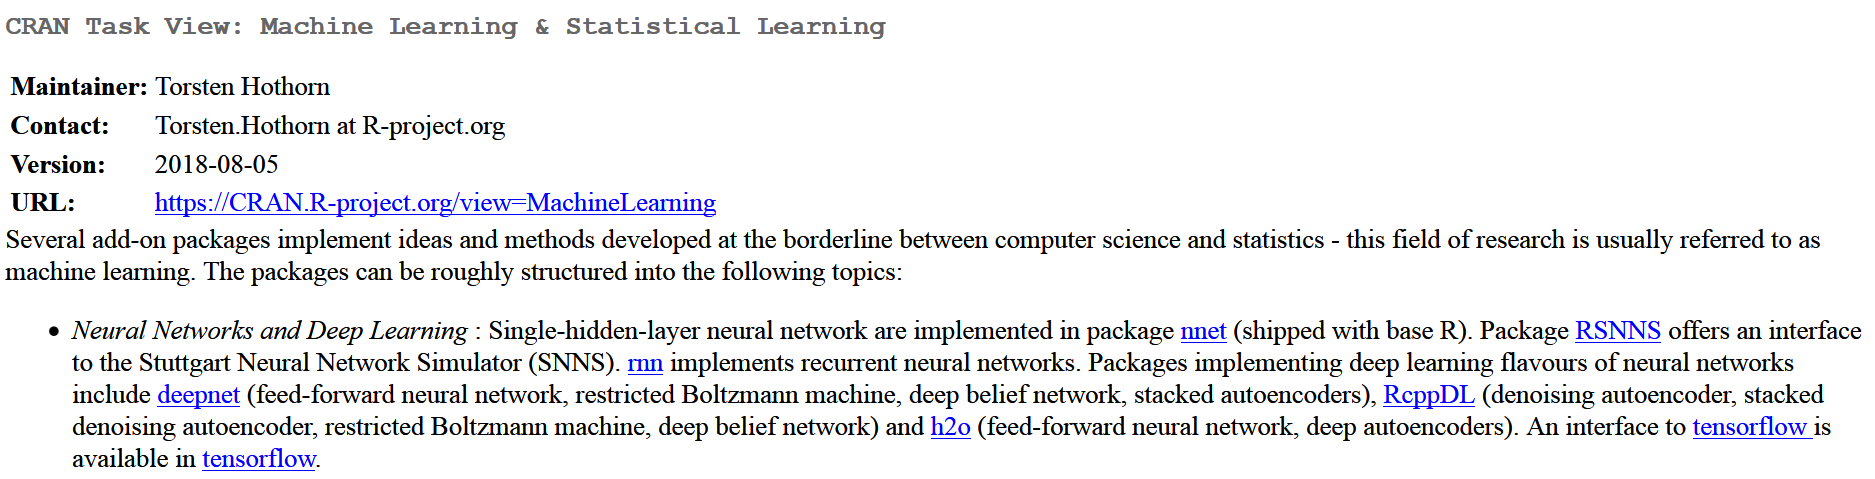
\includegraphics[width=1.10000\textwidth]{figure/taskviewmachinelearning.PNG}
\caption{}
\end{figure}

\subsection{Install all packages of a task
view}\label{install-all-packages-of-a-task-view}

\begin{Shaded}
\begin{Highlighting}[]
\KeywordTok{install.packages}\NormalTok{(}\StringTok{"ctv"}\NormalTok{)}
\NormalTok{ctv}\OperatorTok{::}\KeywordTok{install.views}\NormalTok{(}\StringTok{"MachineLearning"}\NormalTok{)}
\end{Highlighting}
\end{Shaded}

\subsection{Task: Find R-packages}\label{task-find-r-packages}

Go to \url{https://cran.r-project.org/} and search for packages that can
be used:

\begin{itemize}
\tightlist
\item
  to reduce overfitting
\item
  for random forests
\item
  for gradient boosting
\item
  for neural networks
\item
  for clustering
\end{itemize}

\subsection{Preparation - packages}\label{preparation---packages}

\begin{Shaded}
\begin{Highlighting}[]
\KeywordTok{library}\NormalTok{(dplyr)}
\end{Highlighting}
\end{Shaded}

\begin{figure}
\centering
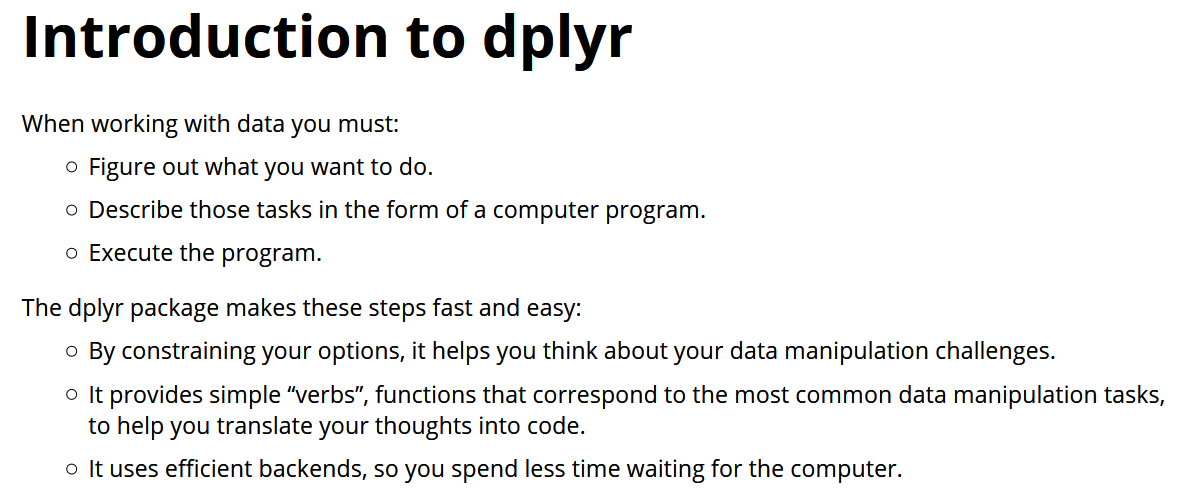
\includegraphics{figure/dplyr_vignette.PNG}
\caption{}
\end{figure}

\begin{Shaded}
\begin{Highlighting}[]
\KeywordTok{library}\NormalTok{(magrittr)}
\end{Highlighting}
\end{Shaded}


\includegraphics{figure/magrittr_vignette.jpg} \#\# Import \texttt{.csv}
data

\subsubsection{\texorpdfstring{The \texttt{read.csv}
command}{The read.csv command}}\label{the-read.csv-command}

\begin{itemize}
\tightlist
\item
  Use \texttt{read.csv2} for German data
\end{itemize}

\begin{Shaded}
\begin{Highlighting}[]
\NormalTok{?read.csv}
\NormalTok{?read.csv2}
\end{Highlighting}
\end{Shaded}

\subsubsection{Using a path to import
data}\label{using-a-path-to-import-data}

\begin{Shaded}
\begin{Highlighting}[]
\NormalTok{path1<-}\StringTok{"https://raw.githubusercontent.com/"}
\NormalTok{path2<-}\StringTok{ "thomaspernet/data_csv_r/master/data/"}
\NormalTok{dname <-}\StringTok{ "titanic_csv.csv"}
\NormalTok{titanic <-}\StringTok{ }\KeywordTok{read.csv}\NormalTok{(}\KeywordTok{paste0}\NormalTok{(path1,path2,dname))}
\end{Highlighting}
\end{Shaded}

\subsubsection{Save the dataset}\label{save-the-dataset}

\begin{Shaded}
\begin{Highlighting}[]
\KeywordTok{save}\NormalTok{(titanic,}\DataTypeTok{file=}\StringTok{"../data/titanic.RData"}\NormalTok{)}
\end{Highlighting}
\end{Shaded}

\subsection{The titanic dataset}\label{the-titanic-dataset}

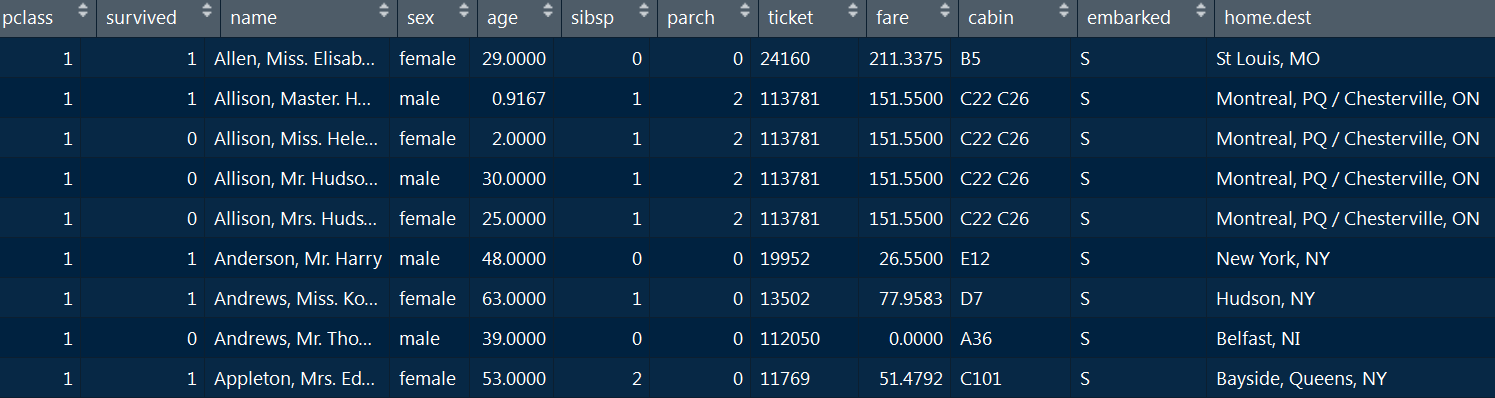
\includegraphics{figure/titanicdata.PNG}

\subsection{\texorpdfstring{The function \texttt{scan} to import
data}{The function scan to import data}}\label{the-function-scan-to-import-data}

\begin{itemize}
\tightlist
\item
  \texttt{scan} has an easy way to distinguish comments from data
\end{itemize}

\begin{Shaded}
\begin{Highlighting}[]
\NormalTok{?scan}
\end{Highlighting}
\end{Shaded}

\subsubsection{Example dataset}\label{example-dataset}

\begin{Shaded}
\begin{Highlighting}[]
\KeywordTok{cat}\NormalTok{(}\StringTok{"TITLE extra line"}\NormalTok{, }\StringTok{"# a comment"}\NormalTok{,}\StringTok{"2 3 5 7"}\NormalTok{, }\StringTok{"11 13 17"}\NormalTok{, }
    \DataTypeTok{file =} \StringTok{"../data/ex.data"}\NormalTok{, }\DataTypeTok{sep =} \StringTok{"}\CharTok{\textbackslash{}n}\StringTok{"}\NormalTok{)}
\end{Highlighting}
\end{Shaded}

\subsubsection{Import data and skip the first
line}\label{import-data-and-skip-the-first-line}

\begin{Shaded}
\begin{Highlighting}[]
\NormalTok{pp<-}\KeywordTok{scan}\NormalTok{(}\StringTok{"../data/ex.data"}\NormalTok{,}\DataTypeTok{skip=}\DecValTok{1}\NormalTok{,}\DataTypeTok{quiet=}\OtherTok{TRUE}\NormalTok{)}
\end{Highlighting}
\end{Shaded}

\begin{Shaded}
\begin{Highlighting}[]
\NormalTok{pp <-}\StringTok{ }\KeywordTok{scan}\NormalTok{(}\StringTok{"../data/ex.data"}\NormalTok{,}\DataTypeTok{comment.char=}\StringTok{"#"}\NormalTok{, }\DataTypeTok{skip =} \DecValTok{1}\NormalTok{,}\DataTypeTok{quiet =} \OtherTok{TRUE}\NormalTok{)}
\end{Highlighting}
\end{Shaded}

\subsection{The download the data from
UCI.}\label{the-download-the-data-from-uci.}

\begin{Shaded}
\begin{Highlighting}[]
\NormalTok{path1 <-}\StringTok{ "http://archive.ics.uci.edu/ml/"}
\NormalTok{path2 <-}\StringTok{ "machine-learning-databases/00243/"}
\NormalTok{dname <-}\StringTok{ 'yacht_hydrodynamics.data'}
\end{Highlighting}
\end{Shaded}

\begin{Shaded}
\begin{Highlighting}[]
\NormalTok{url<-}\StringTok{ }\KeywordTok{paste0}\NormalTok{(path1,path2,dname)}
\NormalTok{Yacht_Data <-}\StringTok{ }\NormalTok{readr}\OperatorTok{::}\KeywordTok{read_table}\NormalTok{(}\DataTypeTok{file =}\NormalTok{ url)}
\end{Highlighting}
\end{Shaded}

\subsection{Built in datasets}\label{built-in-datasets}

\begin{itemize}
\tightlist
\item
  A sample dataset is often provided to demonstrate the functionality of
  a package.
\item
  These records can be loaded using the \texttt{data} command.
\end{itemize}

\begin{Shaded}
\begin{Highlighting}[]
\KeywordTok{data}\NormalTok{(iris)}
\end{Highlighting}
\end{Shaded}

\begin{itemize}
\tightlist
\item
  There is also a
  \href{https://github.com/bquast/datasets.load}{\textbf{RStudio
  Add-In}} that helps to find a built-in dataset.
\end{itemize}

\begin{Shaded}
\begin{Highlighting}[]
\KeywordTok{install.packages}\NormalTok{(}\StringTok{"datasets.load"}\NormalTok{)}
\end{Highlighting}
\end{Shaded}

\subsection{\texorpdfstring{Exkurs
\href{https://cran.r-project.org/web/packages/addinslist/README.html}{RStudio
Addins}}{Exkurs RStudio Addins}}\label{exkurs-rstudio-addins}

\begin{itemize}
\tightlist
\item
  Oben rechts befindet sich ein Button Addins
\end{itemize}

\begin{figure}
\centering

\includegraphics{figure/addins.PNG}
\caption{}
\end{figure}

\begin{figure}
\centering
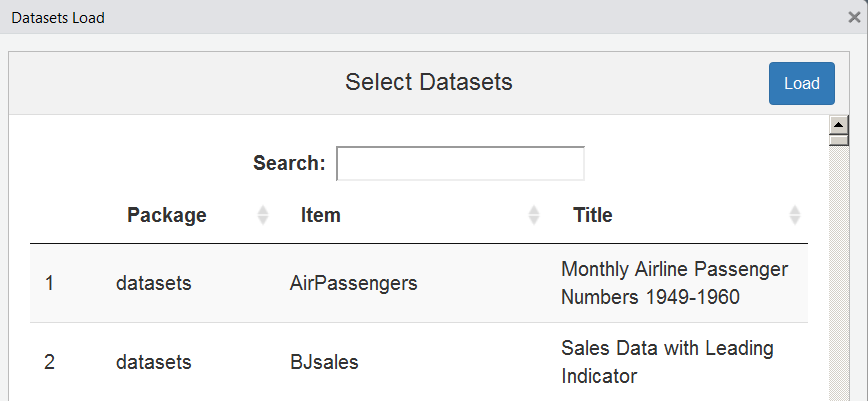
\includegraphics{figure/datasetsload.PNG}
\caption{}
\end{figure}

\subsection{Exercise}\label{exercise}

Load the the built-in dataset \texttt{swiss} and answer the following
questions:

\begin{itemize}
\tightlist
\item
  How many observations and variables are available?
\item
  What is the scale level of the variables?
\end{itemize}

Create an interactive data table

\subsection{\texorpdfstring{The R-package
\texttt{data.table}}{The R-package data.table}}\label{the-r-package-data.table}

\subsubsection{Get an overview}\label{get-an-overview}

\begin{Shaded}
\begin{Highlighting}[]
\KeywordTok{data}\NormalTok{(airquality)}
\KeywordTok{head}\NormalTok{(airquality)}
\end{Highlighting}
\end{Shaded}

\begin{verbatim}
##   Ozone Solar.R Wind Temp Month Day
## 1    41     190  7.4   67     5   1
## 2    36     118  8.0   72     5   2
## 3    12     149 12.6   74     5   3
## 4    18     313 11.5   62     5   4
## 5    NA      NA 14.3   56     5   5
## 6    28      NA 14.9   66     5   6
\end{verbatim}

\subsection{\texorpdfstring{Overview with
\texttt{data.table}}{Overview with data.table}}\label{overview-with-data.table}

\begin{Shaded}
\begin{Highlighting}[]
\KeywordTok{library}\NormalTok{(data.table)}
\NormalTok{(airq <-}\StringTok{ }\KeywordTok{data.table}\NormalTok{(airquality))}
\end{Highlighting}
\end{Shaded}

\begin{verbatim}
##      Ozone Solar.R Wind Temp Month Day
##   1:    41     190  7.4   67     5   1
##   2:    36     118  8.0   72     5   2
##   3:    12     149 12.6   74     5   3
##   4:    18     313 11.5   62     5   4
##   5:    NA      NA 14.3   56     5   5
##  ---                                  
## 149:    30     193  6.9   70     9  26
## 150:    NA     145 13.2   77     9  27
## 151:    14     191 14.3   75     9  28
## 152:    18     131  8.0   76     9  29
## 153:    20     223 11.5   68     9  30
\end{verbatim}

\subsection{How to get help}\label{how-to-get-help}

\begin{itemize}
\tightlist
\item
  I use \href{figure/duckduckgo.PNG}{\textbf{duckduckgo:}}
\end{itemize}

\begin{verbatim}
R-project + "what I want to know" 
\end{verbatim}

\begin{itemize}
\tightlist
\item
  this works of course for all search engines!
\end{itemize}

\begin{figure}
\centering

\includegraphics{figure/duckduckgo.PNG}
\caption{}
\end{figure}

\subsection{\texorpdfstring{\href{https://www.datacamp.com/community/tutorials/pipe-r-tutorial}{Exercise}}{Exercise}}\label{exercise-1}

\begin{itemize}
\tightlist
\item
  Draw 8 random numbers from the uniform distribution and save them in a
  vector \texttt{x}
\item
  Compute the logarithm of \texttt{x}, return suitably lagged and
  iterated differences,
\item
  compute the exponential function and round the result
\end{itemize}

\begin{verbatim}
## [1]  0.0  5.5  0.9  2.5  0.0 44.1  1.1
\end{verbatim}

\subsection{\texorpdfstring{\href{https://www.datacamp.com/community/tutorials/pipe-r-tutorial}{The
pipe operator}}{The pipe operator}}\label{the-pipe-operator}

\begin{Shaded}
\begin{Highlighting}[]
\KeywordTok{library}\NormalTok{(magrittr)}

\CommentTok{# Perform the same computations on `x` as above}
\NormalTok{x }\OperatorTok\StringTok{ }\KeywordTok{log}\NormalTok{() }\OperatorTok
\StringTok{    }\KeywordTok{diff}\NormalTok{() }\OperatorTok
\StringTok{    }\KeywordTok{exp}\NormalTok{() }\OperatorTok
\StringTok{    }\KeywordTok{round}\NormalTok{(}\DecValTok{1}\NormalTok{)}
\end{Highlighting}
\end{Shaded}

\begin{verbatim}
## [1]  0.0  5.5  0.9  2.5  0.0 44.1  1.1
\end{verbatim}

\subsection{How to deal with missing
values}\label{how-to-deal-with-missing-values}

\begin{Shaded}
\begin{Highlighting}[]
\NormalTok{?na.omit}
\end{Highlighting}
\end{Shaded}

\begin{Shaded}
\begin{Highlighting}[]
\NormalTok{airq}
\end{Highlighting}
\end{Shaded}

\begin{verbatim}
##      Ozone Solar.R Wind Temp Month Day
##   1:    41     190  7.4   67     5   1
##   2:    36     118  8.0   72     5   2
##   3:    12     149 12.6   74     5   3
##   4:    18     313 11.5   62     5   4
##   5:    NA      NA 14.3   56     5   5
##  ---                                  
## 149:    30     193  6.9   70     9  26
## 150:    NA     145 13.2   77     9  27
## 151:    14     191 14.3   75     9  28
## 152:    18     131  8.0   76     9  29
## 153:    20     223 11.5   68     9  30
\end{verbatim}

\subsection{\texorpdfstring{The command
\texttt{na.omit}}{The command na.omit}}\label{the-command-na.omit}

\begin{Shaded}
\begin{Highlighting}[]
\KeywordTok{na.omit}\NormalTok{(airq)}
\end{Highlighting}
\end{Shaded}

\begin{verbatim}
##      Ozone Solar.R Wind Temp Month Day
##   1:    41     190  7.4   67     5   1
##   2:    36     118  8.0   72     5   2
##   3:    12     149 12.6   74     5   3
##   4:    18     313 11.5   62     5   4
##   5:    23     299  8.6   65     5   7
##  ---                                  
## 107:    14      20 16.6   63     9  25
## 108:    30     193  6.9   70     9  26
## 109:    14     191 14.3   75     9  28
## 110:    18     131  8.0   76     9  29
## 111:    20     223 11.5   68     9  30
\end{verbatim}

\subsection{\texorpdfstring{\href{https://www.guru99.com/r-decision-trees.html}{Clean
the titanic data
set}}{Clean the titanic data set}}\label{clean-the-titanic-data-set}

\begin{Shaded}
\begin{Highlighting}[]
\NormalTok{clean_titanic <-}\StringTok{ }\NormalTok{titanic }\OperatorTok\StringTok{    }
\StringTok{  }\KeywordTok{mutate}\NormalTok{(}\DataTypeTok{pclass=}\KeywordTok{factor}\NormalTok{(pclass,}\DataTypeTok{levels =} \KeywordTok{c}\NormalTok{(}\DecValTok{1}\NormalTok{, }\DecValTok{2}\NormalTok{, }\DecValTok{3}\NormalTok{),}
                       \DataTypeTok{labels=}\KeywordTok{c}\NormalTok{(}\StringTok{'Upper'}\NormalTok{,}\StringTok{'Middle'}\NormalTok{,}\StringTok{'Lower'}\NormalTok{)),}
    \DataTypeTok{survived =} \KeywordTok{factor}\NormalTok{(survived,}\DataTypeTok{levels =} \KeywordTok{c}\NormalTok{(}\DecValTok{0}\NormalTok{, }\DecValTok{1}\NormalTok{), }
                      \DataTypeTok{labels=}\KeywordTok{c}\NormalTok{(}\StringTok{'No'}\NormalTok{, }\StringTok{'Yes'}\NormalTok{))) }\OperatorTok
\KeywordTok{na.omit}\NormalTok{()}
\end{Highlighting}
\end{Shaded}

\subsubsection{\texorpdfstring{\texttt{mutate(pclass\ =\ factor(...}:}{mutate(pclass = factor(...:}}\label{mutatepclass-factor...}

\begin{itemize}
\tightlist
\item
  Add label to the variable pclass.
\item
  1 becomes Upper, 2 becomes MIddle and 3 becomes lower
\end{itemize}

\subsubsection{\texorpdfstring{\texttt{factor(survived,...}:}{factor(survived,...:}}\label{factorsurvived...}

\begin{itemize}
\item
  Add label to the variable survived.
\item
  1 Becomes No and 2 becomes Yes
\item
  \texttt{na.omit()}: Remove the NA observations
\end{itemize}

\subsection{Get an overview of the
data}\label{get-an-overview-of-the-data}

\begin{Shaded}
\begin{Highlighting}[]
\KeywordTok{glimpse}\NormalTok{(clean_titanic)}
\end{Highlighting}
\end{Shaded}

\begin{verbatim}
## Observations: 1,045
## Variables: 13
## $ X         <int> 1, 2, 3, 4, 5, 6, 7, 8, 9, 10, 11, 12, 13, 14, 15, 1...
## $ pclass    <fct> Upper, Upper, Upper, Upper, Upper, Upper, Upper, Upp...
## $ survived  <fct> Yes, Yes, No, No, No, Yes, Yes, No, Yes, No, No, Yes...
## $ name      <fct> "Allen, Miss. Elisabeth Walton", "Allison, Master. H...
## $ sex       <fct> female, male, female, male, female, male, female, ma...
## $ age       <dbl> 29.0000, 0.9167, 2.0000, 30.0000, 25.0000, 48.0000, ...
## $ sibsp     <int> 0, 1, 1, 1, 1, 0, 1, 0, 2, 0, 1, 1, 0, 0, 0, 0, 0, 0...
## $ parch     <int> 0, 2, 2, 2, 2, 0, 0, 0, 0, 0, 0, 0, 0, 0, 0, 1, 1, 0...
## $ ticket    <fct> 24160, 113781, 113781, 113781, 113781, 19952, 13502,...
## $ fare      <dbl> 211.3375, 151.5500, 151.5500, 151.5500, 151.5500, 26...
## $ cabin     <fct> B5, C22 C26, C22 C26, C22 C26, C22 C26, E12, D7, A36...
## $ embarked  <fct> S, S, S, S, S, S, S, S, S, C, C, C, C, S, S, C, C, C...
## $ home.dest <fct> "St Louis, MO", "Montreal, PQ / Chesterville, ON", "...
\end{verbatim}

\subsection{\texorpdfstring{\href{https://datascienceplus.com/fitting-neural-network-in-r/}{Example
Data - Housing Values in Suburbs of
Boston}}{Example Data - Housing Values in Suburbs of Boston}}\label{example-data---housing-values-in-suburbs-of-boston}

\begin{Shaded}
\begin{Highlighting}[]
\KeywordTok{library}\NormalTok{(MASS)}
\NormalTok{bdat <-}\StringTok{ }\NormalTok{Boston}
\end{Highlighting}
\end{Shaded}

\begin{figure}
\centering
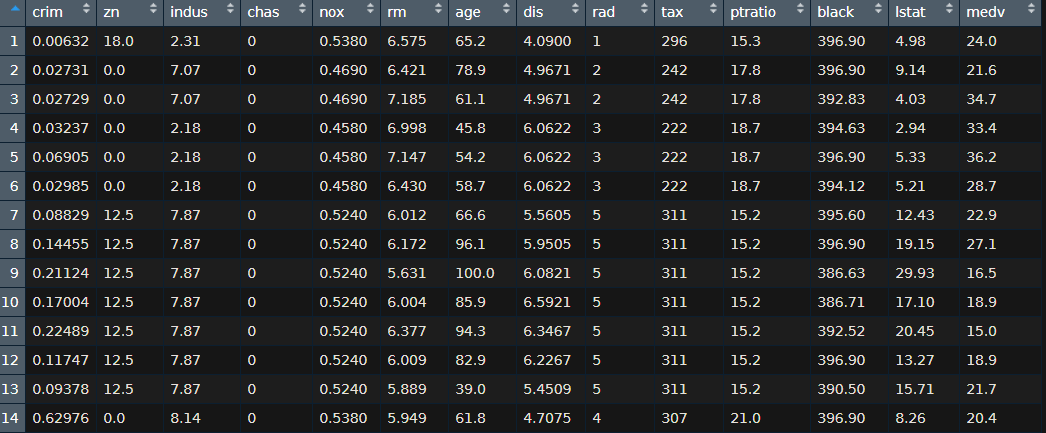
\includegraphics{figure/bostondata.PNG}
\caption{}
\end{figure}

\subsection{Normalize your data}\label{normalize-your-data}

\subsubsection{Compute maximum and minimum per
column}\label{compute-maximum-and-minimum-per-column}

\begin{Shaded}
\begin{Highlighting}[]
\NormalTok{maxs <-}\StringTok{ }\KeywordTok{apply}\NormalTok{(bdat, }\DecValTok{2}\NormalTok{, max) }
\NormalTok{mins <-}\StringTok{ }\KeywordTok{apply}\NormalTok{(bdat, }\DecValTok{2}\NormalTok{, min)}
\end{Highlighting}
\end{Shaded}

\subsubsection{\texorpdfstring{\texttt{scale} - Scaling and Centering of
Matrix-like
Objects}{scale - Scaling and Centering of Matrix-like Objects}}\label{scale---scaling-and-centering-of-matrix-like-objects}

\begin{Shaded}
\begin{Highlighting}[]
\NormalTok{scaled <-}\StringTok{ }\KeywordTok{as.data.frame}\NormalTok{(}\KeywordTok{scale}\NormalTok{(bdat, }\DataTypeTok{center =}\NormalTok{ mins, }
                              \DataTypeTok{scale =}\NormalTok{ maxs }\OperatorTok{-}\StringTok{ }\NormalTok{mins))}
\end{Highlighting}
\end{Shaded}

\subsection{The scaled data}\label{the-scaled-data}

\begin{figure}
\centering
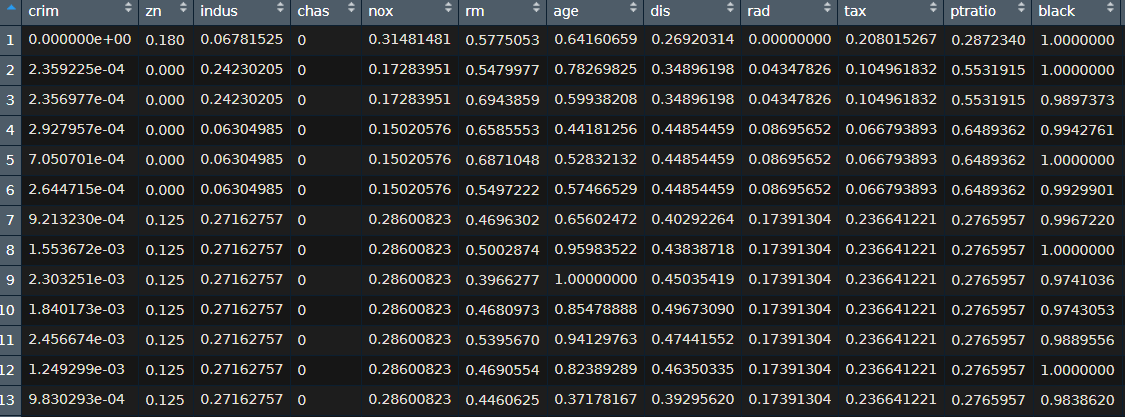
\includegraphics{figure/bostonscaled.PNG}
\caption{}
\end{figure}

\subsection{\texorpdfstring{The command
\texttt{sample}}{The command sample}}\label{the-command-sample}

\begin{itemize}
\tightlist
\item
  We can use this command to draw a sample.
\item
  We need the command later to split our dataset into a test and a
  training dataset.
\end{itemize}

\begin{Shaded}
\begin{Highlighting}[]
\KeywordTok{sample}\NormalTok{(}\DecValTok{1}\OperatorTok{:}\DecValTok{10}\NormalTok{,}\DecValTok{3}\NormalTok{,}\DataTypeTok{replace=}\NormalTok{T)}
\end{Highlighting}
\end{Shaded}

\begin{verbatim}
## [1] 3 6 3
\end{verbatim}

\begin{Shaded}
\begin{Highlighting}[]
\KeywordTok{sample}\NormalTok{(}\DecValTok{1}\OperatorTok{:}\DecValTok{10}\NormalTok{,}\DecValTok{3}\NormalTok{,}\DataTypeTok{replace=}\NormalTok{T)}
\end{Highlighting}
\end{Shaded}

\begin{verbatim}
## [1]  5 10  7
\end{verbatim}

\subsection{Set a seed}\label{set-a-seed}

\begin{itemize}
\tightlist
\item
  \texttt{set.seed} is the recommended way to specify seeds.
\item
  If we set a seed, we get the same result for random events.
\item
  This function is mainly required for simulations.
\end{itemize}

\begin{Shaded}
\begin{Highlighting}[]
\KeywordTok{set.seed}\NormalTok{(}\DecValTok{234}\NormalTok{)}
\KeywordTok{sample}\NormalTok{(}\DecValTok{1}\OperatorTok{:}\DecValTok{10}\NormalTok{,}\DecValTok{3}\NormalTok{,}\DataTypeTok{replace=}\NormalTok{T)}
\end{Highlighting}
\end{Shaded}

\begin{verbatim}
## [1] 8 8 1
\end{verbatim}

\begin{Shaded}
\begin{Highlighting}[]
\KeywordTok{set.seed}\NormalTok{(}\DecValTok{234}\NormalTok{)}
\KeywordTok{sample}\NormalTok{(}\DecValTok{1}\OperatorTok{:}\DecValTok{10}\NormalTok{,}\DecValTok{3}\NormalTok{,}\DataTypeTok{replace=}\NormalTok{T)}
\end{Highlighting}
\end{Shaded}

\begin{verbatim}
## [1] 8 8 1
\end{verbatim}

\subsection{\texorpdfstring{\href{https://www.r-bloggers.com/5-ways-to-measure-running-time-of-r-code/}{Time
measurement}}{Time measurement}}\label{time-measurement}

\begin{Shaded}
\begin{Highlighting}[]
\NormalTok{start_time <-}\StringTok{ }\KeywordTok{Sys.time}\NormalTok{()}
\NormalTok{ab <-}\StringTok{ }\KeywordTok{runif}\NormalTok{(}\DecValTok{10000000}\NormalTok{)}
\NormalTok{end_time <-}\StringTok{ }\KeywordTok{Sys.time}\NormalTok{()}

\NormalTok{end_time }\OperatorTok{-}\StringTok{ }\NormalTok{start_time}
\end{Highlighting}
\end{Shaded}

\begin{verbatim}
## Time difference of 0.3051941 secs
\end{verbatim}

\subsection{How many cores are
available}\label{how-many-cores-are-available}

\begin{Shaded}
\begin{Highlighting}[]
\KeywordTok{library}\NormalTok{(doParallel)}
\KeywordTok{detectCores}\NormalTok{()}
\end{Highlighting}
\end{Shaded}

\begin{verbatim}
## [1] 4
\end{verbatim}

\subsection{Make cluster}\label{make-cluster}

\begin{Shaded}
\begin{Highlighting}[]
\NormalTok{cl <-}\StringTok{ }\KeywordTok{makeCluster}\NormalTok{(}\KeywordTok{detectCores}\NormalTok{())}
\KeywordTok{registerDoParallel}\NormalTok{(cl)}
\end{Highlighting}
\end{Shaded}

\begin{Shaded}
\begin{Highlighting}[]
\NormalTok{start_time <-}\StringTok{ }\KeywordTok{Sys.time}\NormalTok{()}
\NormalTok{ab <-}\StringTok{ }\KeywordTok{runif}\NormalTok{(}\DecValTok{10000000}\NormalTok{)}
\NormalTok{end_time <-}\StringTok{ }\KeywordTok{Sys.time}\NormalTok{()}

\NormalTok{end_time }\OperatorTok{-}\StringTok{ }\NormalTok{start_time}
\end{Highlighting}
\end{Shaded}

\begin{verbatim}
## Time difference of 0.3033919 secs
\end{verbatim}

\begin{Shaded}
\begin{Highlighting}[]
\KeywordTok{stopCluster}\NormalTok{(cl)}
\end{Highlighting}
\end{Shaded}

\begin{Shaded}
\begin{Highlighting}[]
\NormalTok{?parallel}\OperatorTok{::}\NormalTok{makeCluster}
\end{Highlighting}
\end{Shaded}

\subsection{Resources}\label{resources}

\begin{itemize}
\tightlist
\item
  \href{https://github.com/DataScienceSpecialization/courses}{\textbf{Course
  materials for the Data Science Specialization}}
\item
  Data wrangling -
  \href{https://cran.r-project.org/web/packages/dplyr/vignettes/dplyr.html}{\textbf{\texttt{dplyr}
  vignette}} -
\item
  The usage of pipes -
  \href{https://cran.r-project.org/web/packages/magrittr/vignettes/magrittr.html}{\textbf{\texttt{magrittr}
  vignette}} 
\end{itemize}


\end{document}
